Das Beidseitige Layout und der entsprechende Schaltplan der kalten Elektronik aus Abb. \ref{fig:ElektronikBilder} sind in Abb. \ref{fig:Layout} und Abb. \ref{fig:Schaltplan} dargestellt.
Das Layout und der Schaltplan entsprechen nicht vollständig der kalten Elektronik mit welchen die Daten aufgenommen wurden.
Manuel wurde durch mechanische Einwirkung der Schaltplan entsprechend Abb. \ref{fig:Ausleseelektronik} verwirklicht.

\begin{figure}[!b]
\begin{center}
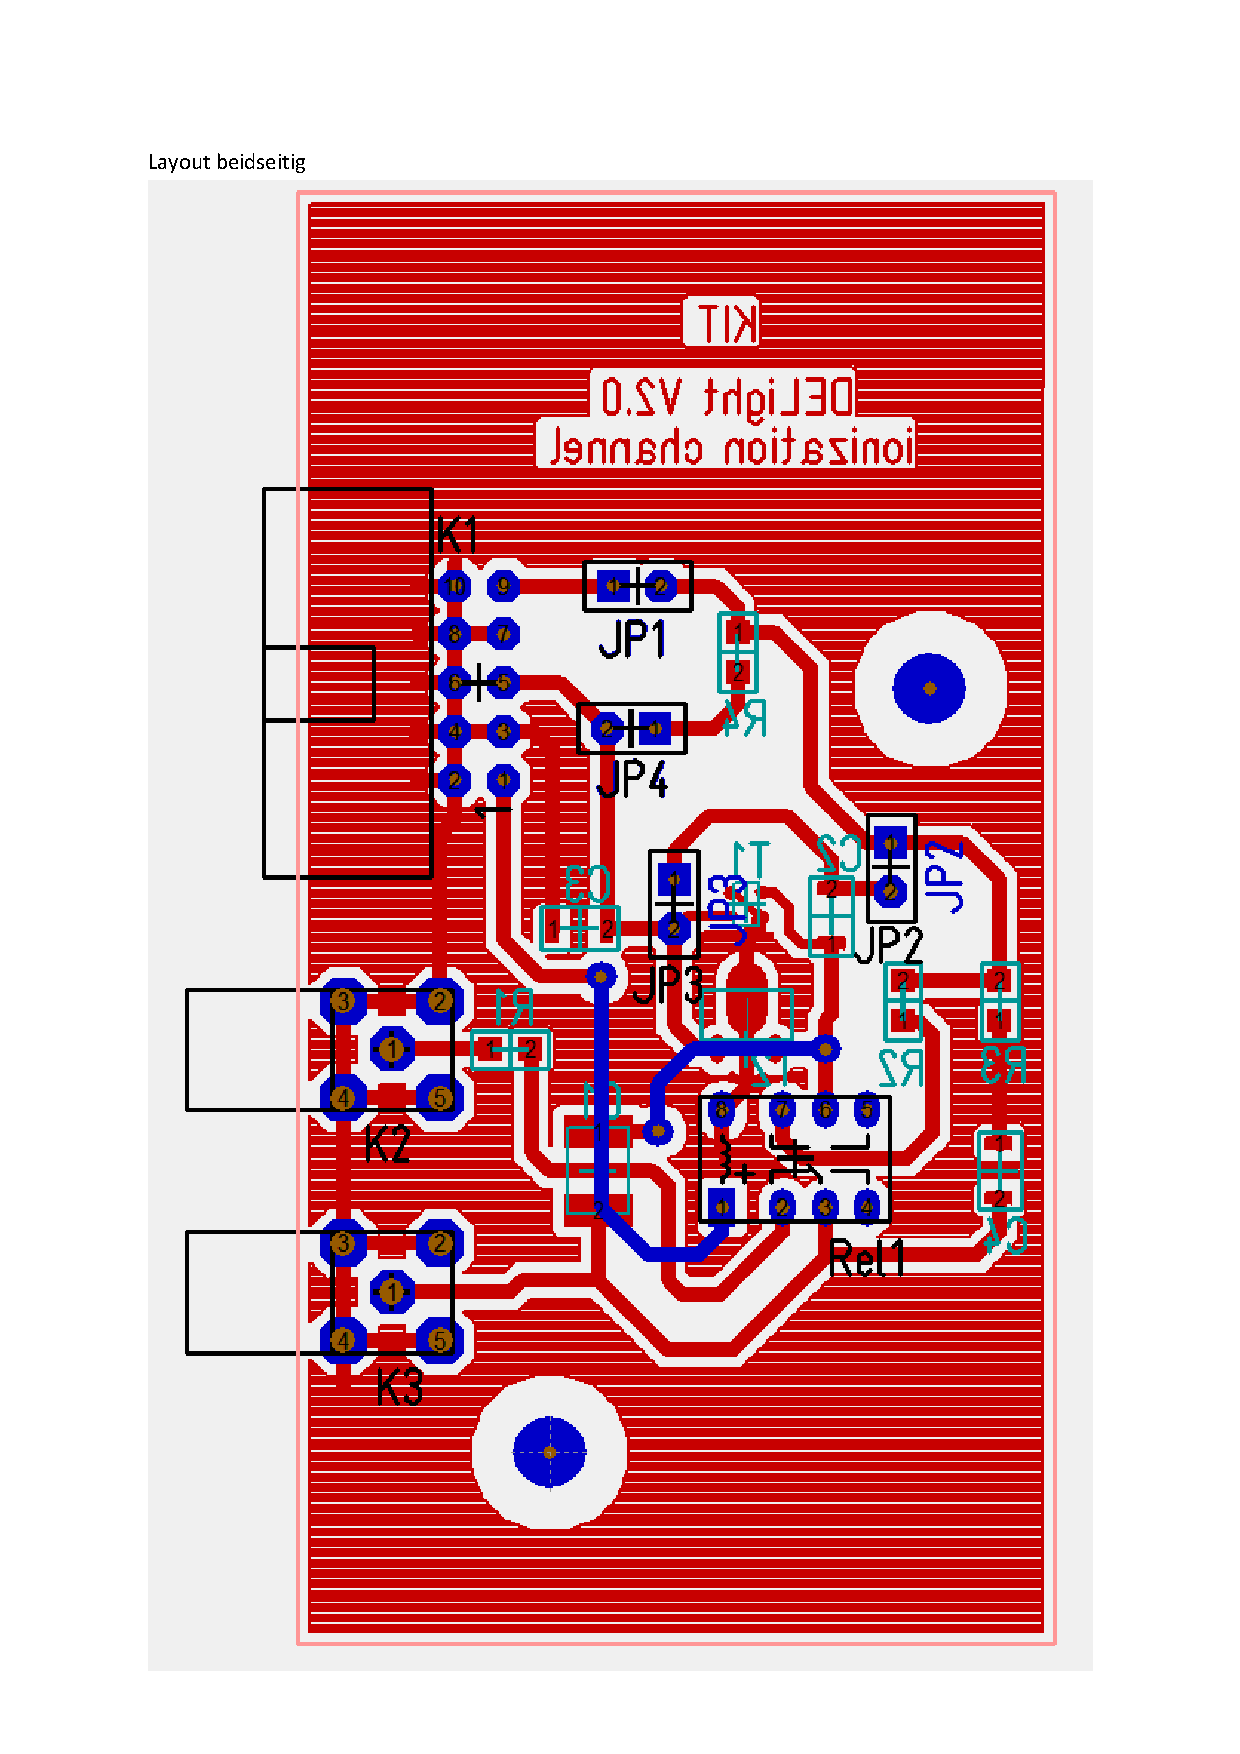
\includegraphics[page=1,width=\textwidth]{./fig/SchaltplanLayoutV2.pdf}
\vspace{-0.5cm}
\caption{Layout der kalten Elektronik}
\label{fig:Layout}
\end{center}
\end{figure}
\begin{figure}[!b]
\begin{center}
\includegraphics[page=6,width=\textwidth]{./fig/SchaltplanLayoutV2.pdf}
\vspace{-0.5cm}
\caption{Schaltplan der kalten Elektronik}
\label{fig:Schaltplan}
\end{center}
\end{figure}